\documentclass{article}
\usepackage[utf8]{inputenc}
\usepackage{graphicx}

\usepackage{hyperref}
\hypersetup{
    colorlinks=true,
    linkcolor=blue,
    filecolor=magenta,      
    urlcolor=cyan,
}
 
\urlstyle{same}

\title{Elaboration Plan}
\author{Lauren Franks}
\date{FOAR705}

\begin{document}

\maketitle
\tableofcontents
\section{Objective}

As identified in my scoping document, my overall objective is to develop social awareness and understanding of dataveillance processes and effects. I will achieve this by:
\begin{itemize}
\item Finding and deploying a set of privacy extensions for my browser to secure my personal data.
\item Presenting my findings on a publicly accessible digital platform.
\end{itemize}

\section{Technologies Identified}
\subsection{Browser privacy extensions}

 
\href{https://github.com/gorhill/uBlock}{uBlock Origin v1.21.6}

Developed by Raymond Hill (2014), uBlock Origin is an adblocker with a high level of customisability and seems to offer plenty of information about its processes. This will be important for my project as I will need to be able to articulate what each component of the software achieves. Furthermore, other adblocking extensions such as \href{https://getadblock.com/}{Ablock} trade transparency regarding functionality for simple user interface aesthetics, which can mask nefarious capabilities.\newline


\noindent\href{https://github.com/gorhill/uMatrix}{uMatrix v1.3.16}

Also developed by Raymond Hill (2014), uMatrix blocks all third-party scripts by default until you unblock the site. Like uBlock Origin it seems to offer extensive customisation and transparency. It is not as intuitive to use as uBlock Origin, for example I have been unable to access my emails and have had to disable uMatrix until I figure out how to use whitelisting functions.\newline

\noindent\href{https://trockerapp.github.io/}{Trocker v2.6.1}

Trocker is an extension that blocks pixel tracking in emails. This may be unnecessary if it turns out that the above extensions are able to counter pixel tracking as effectively. \newline

\noindent\href{https://www.torproject.org/}{The Tor Project} (not technically an extension)

The Tor Project or simply ‘Tor’ is an opensource browser that counters online surveillance by relying on ‘onion routing’ which routes internet traffic through multiple servers and encrypts it at each point. Unlike Virtual Private Networks (VPNs) that require you invest faith, personal information, and oftentimes money, Tor is free, run by a network of volunteers rather than a single organisation, and allows you to communicate anonymously as soon as you open the browser.    

\subsection{Digital presentation platform}
\href{https://pages.github.com/}{GitHub Pages}

Github Pages allows you to create a static, publicly accessible webpage from a GitHub repository. Uses some HTML language and it also supports \href{https://github.com/jekyll/jekyll}{Jekyll}, an open source tool used within GitHub Pages that transforms plain text files into websites and supports templates and drafts. 

\section{Testing and Revising Identified Technologies}
\subsection{Browser privacy extensions}
I have tested the technologies previously identified to determine if they will protect my personal data from being accessed by third parties, and to determine their ease of use.\newline
 
\noindent\href{https://github.com/gorhill/uBlock}{uBlock Origin v1.21.6}

\noindent Transparency:

According to uBlock Origin's \href{https://github.com/gorhill/uBlock/wiki/Privacy-policy}{privacy policy} uBlock Origin does not collect any data of any kind. It has no home server, it does not embed any kind of analytic hooks in its code, and it does not accept donations or any other form of financing. It is an open source software and the code is publicly available on Github. The logger allows you to see all hidden network requests including ones made by the software, which it uses to update it's filter lists on Github. \newline

\noindent Features:

The default settings of uBlock Origin automatically blocks ads, trackers and malware sites. You can turn it it off on any web page (white-listing it) by clicking the large blue on/off button. The 'zapper function' allows you to temporarily remove a particular item in a web-page such as an image, and the 'filter function' allows you to permanently remove an item so it won't reappear when the page is reloaded. The 'logger' allows you to view real-time network traffic within the browser. I have tried out all of these functions on several websites and they work as anticipated. 

\begin{figure}[htp]
    \centering
    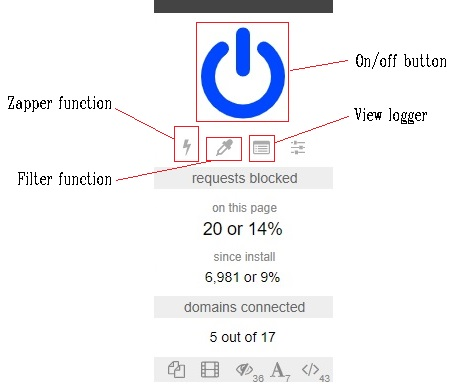
\includegraphics[width=10cm]{Functions labeled.jpg}
    \caption{uBlock Origin dashboard - basic functions}
    \label{fig:uBlock Origin dashboard}
\end{figure}

\noindent Limitations: \newline

Like all privacy software, uBlock Origin relies on filter lists that contain lists of known third-party trackers. These lists are always being updated by users, but it also means that your privacy is compromised if you encounter a new or unknown third-party tracker.\newline
\newline
\noindent\href{https://github.com/gorhill/uMatrix}{uMatrix v1.3.16}

Given that uMatrix is a more complicated software and uBlock Origin will be able to accomplish my privacy objectives, I have decided not to proceed with testing uMatrix.\newline


\noindent\href{https://trockerapp.github.io/}{Trocker v2.6.1}

\noindent Transparency:

Like uBlock Origin, Trocker is an open source software and the code is publicly available on Github. It runs locally and does not send or receive any information through the internet. \newline

\noindent Features: Trocker automatically identifies when a tracking image is injected into an email and blocks it from loading. It successfully blocked images loading in my email accounts and told me how many tracking images each email had. 

\begin{figure}[htp]
    \centering
    
\includegraphics[width=16cm]{trocker ymail block.jpg}
    \caption{Trocker blocking tracking pixels in my Yahoo Mail}
    \label{fig:uBlock Origin dashboard}
\end{figure}


 \newline

\noindent\href{https://www.torproject.org/}{The Tor Project}

on I have decided not to test Tor as it goes beyond the scope of my objectives.

\subsection{Digital presentation platform}
\href{https://pages.github.com/}{GitHub Pages}

I was able to successfully create a very basic static webpage using GitHub Pages, viewable \href{https://laurenfranks11.github.io./}{here.} 

\section{Conclusion and Next Steps}
I have identified and tested three technologies, uBlock Origin, Trocker and GitHub Pages. Together they can conceivably accomplish my goal to to develop social awareness and understanding of dataveillance processes and effects.

The next step will be to write my article further elucidating how privacy is compromised online and how uBlock Origin and Trocker function to protect privacy. I will then use GitHub pages to present my

\end{document}
 article.